% ============================================================
% 第8章：函数的四大性质 + 复合与反函数
% ============================================================

\chapter{函数的四大性质——单调·奇偶·周期·有界}

\begin{applicationbox}
\textbf{学完本章你能做什么？}
\begin{enumerate}
  \item 系统掌握函数的四大性质——\textbf{单调性、奇偶性、周期性、有界性}
  \item 理解\textbf{复合函数}的"链式"结构和\textbf{反函数}的对称性
  \item 标志第0编"函数基础重建"的收官——你已经为数学分析做好了全部准备！
\end{enumerate}
\end{applicationbox}


% ============================================================
\section{从第7章来——总结与升华}
% ============================================================

前7章我们一一认识了各种函数：幂函数、指数函数、对数函数、三角函数。

这一章我们回到\textbf{函数本身}，系统地学习函数的四大基本性质。
这些性质不是某个函数特有的——\textbf{每个函数都可以从这四个维度来分析}。

\begin{center}
\fcolorbox{teal!50}{teal!5}{\parbox{0.85\textwidth}{
\textbf{函数的四大性质：}
\[
\text{单调性} \;\longrightarrow\; \text{增长还是衰减？}
\]
\[
\text{奇偶性} \;\longrightarrow\; \text{对称还是不对称？}
\]
\[
\text{周期性} \;\longrightarrow\; \text{重复还是不重复？}
\]
\[
\text{有界性} \;\longrightarrow\; \text{在范围内还是无限延伸？}
\]
}}
\end{center}


% ============================================================
\section{单调性——递增还是递减？}
% ============================================================

\begin{definitionbox}[单调性]
设函数 \(f(x)\) 在区间 \(I\) 上有定义。
\begin{itemize}
  \item 如果对任意 \(x_1 < x_2\) 都有 \(f(x_1) < f(x_2)\)，则称 \(f\) 在 \(I\) 上\textbf{单调递增}
  \item 如果对任意 \(x_1 < x_2\) 都有 \(f(x_1) > f(x_2)\)，则称 \(f\) 在 \(I\) 上\textbf{单调递减}
\end{itemize}
\end{definitionbox}

\begin{examplebox}[1——单调性直观对比]
\begin{center}
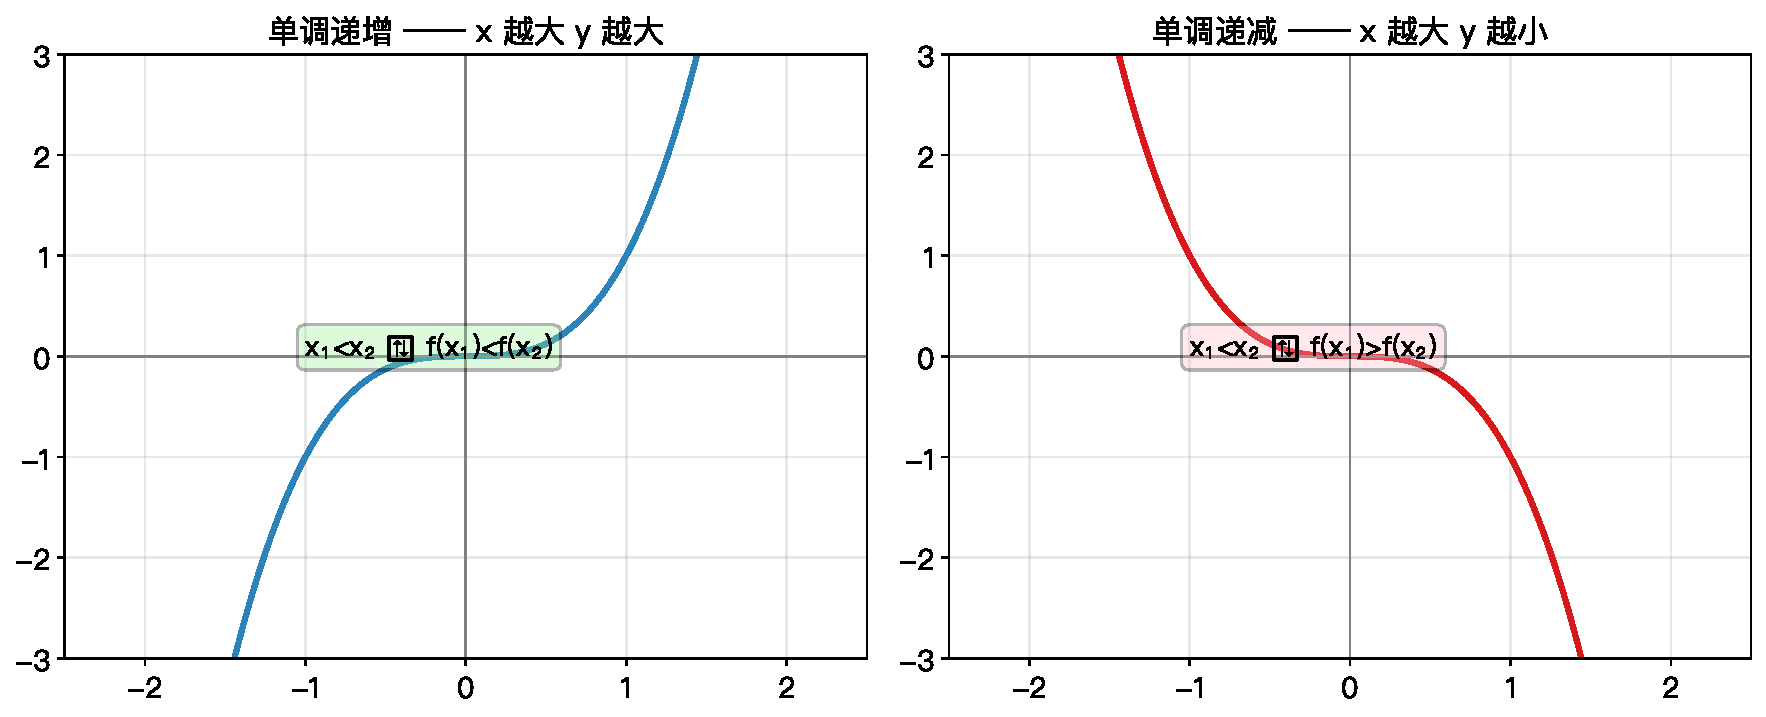
\includegraphics[width=0.85\textwidth]{figures/ch08_monotonic.pdf}
\end{center}

\textbf{左图}（\(y = x^3\)）：从左到右一路向上——单调递增。\\
\textbf{右图}（\(y = -x^3\)）：从左到右一路向下——单调递减。
\end{examplebox}

\begin{examplebox}[2——判断单调性]
判断 \(f(x) = 2^x\) 的单调性。

解：取任意 \(x_1 < x_2\)，则 \(2^{x_1} < 2^{x_2}\)（因为底数 \(2>1\)）。
所以 \(f(x_1) < f(x_2)\) \(\rightarrow\) \textbf{单调递增}。

判断 \(f(x) = (1/2)^x\) 的单调性：
取任意 \(x_1 < x_2\)，则 \((1/2)^{x_1} > (1/2)^{x_2}\)（因为底数 \(1/2 < 1\)）。
所以 \(f(x_1) > f(x_2)\) \(\rightarrow\) \textbf{单调递减}。
\end{examplebox}


% ============================================================
\section{奇偶性——对称还是不对称？}
% ============================================================

\begin{definitionbox}[奇偶性]
设函数 \(f(x)\) 的定义域关于原点对称。
\begin{itemize}
  \item 如果 \(f(-x) = f(x)\) 对所有 \(x\) 成立，则称 \(f\) 是\textbf{偶函数}（关于 \(y\) 轴对称）
  \item 如果 \(f(-x) = -f(x)\) 对所有 \(x\) 成立，则称 \(f\) 是\textbf{奇函数}（关于原点对称）
\end{itemize}
\end{definitionbox}

\begin{examplebox}[3——常见函数的奇偶性]
\begin{center}
\begin{tabular}{c|c|c}
\textbf{奇函数} & \textbf{偶函数} & \textbf{非奇非偶} \\
\hline
\(x\)、\(x^3\)、\(x^5\) & \(x^2\)、\(x^4\)、\(|x|\) & \(2^x\) \\
\(\sin x\)、\(\tan x\)、\(\arcsin x\) & \(\cos x\)、\(\ln|x|\) & \(\log_2 x\) \\
\(\dfrac{1}{x}\) & 常数函数 & \(x+1\) \\
\end{tabular}
\end{center}

\textbf{检验方法：} 把 \(-x\) 代入函数，看结果和 \(f(x)\) 还是 \(-f(x)\) 相等。
\end{examplebox}


% ============================================================
\section{周期性——重复还是不重复？}
% ============================================================

\begin{definitionbox}[周期性]
如果存在非零常数 \(T\)，使得对定义域内的所有 \(x\) 都有
\[
f(x + T) = f(x)
\]
则称 \(f\) 是\textbf{周期函数}，\(T\) 是它的一个周期。
最小的正周期叫\textbf{最小正周期}。
\end{definitionbox}

\begin{examplebox}[4——周期函数举例]
\begin{center}
\begin{tabular}{c|c}
\textbf{函数} & \textbf{最小正周期} \\
\hline
\(\sin x\)、\(\cos x\) & \(2\pi\) \\
\(\tan x\) & \(\pi\) \\
常数函数 & 任意数都是周期（但没有最小正周期） \\
\end{tabular}
\end{center}

\textbf{注意：} 幂函数、指数函数、对数函数都不是周期函数。
周期性是三角函数特有的性质。
\end{examplebox}


% ============================================================
\section{有界性——在范围内还是无限延伸？}
% ============================================================

\begin{definitionbox}[有界性]
如果存在一个常数 \(M > 0\)，使得对定义域内的所有 \(x\) 都有
\[
|f(x)| \le M
\]
则称 \(f\) 是\textbf{有界函数}。否则称 \(f\) 是\textbf{无界函数}。
\end{definitionbox}

\begin{examplebox}[5——有界 vs 无界]
\begin{center}
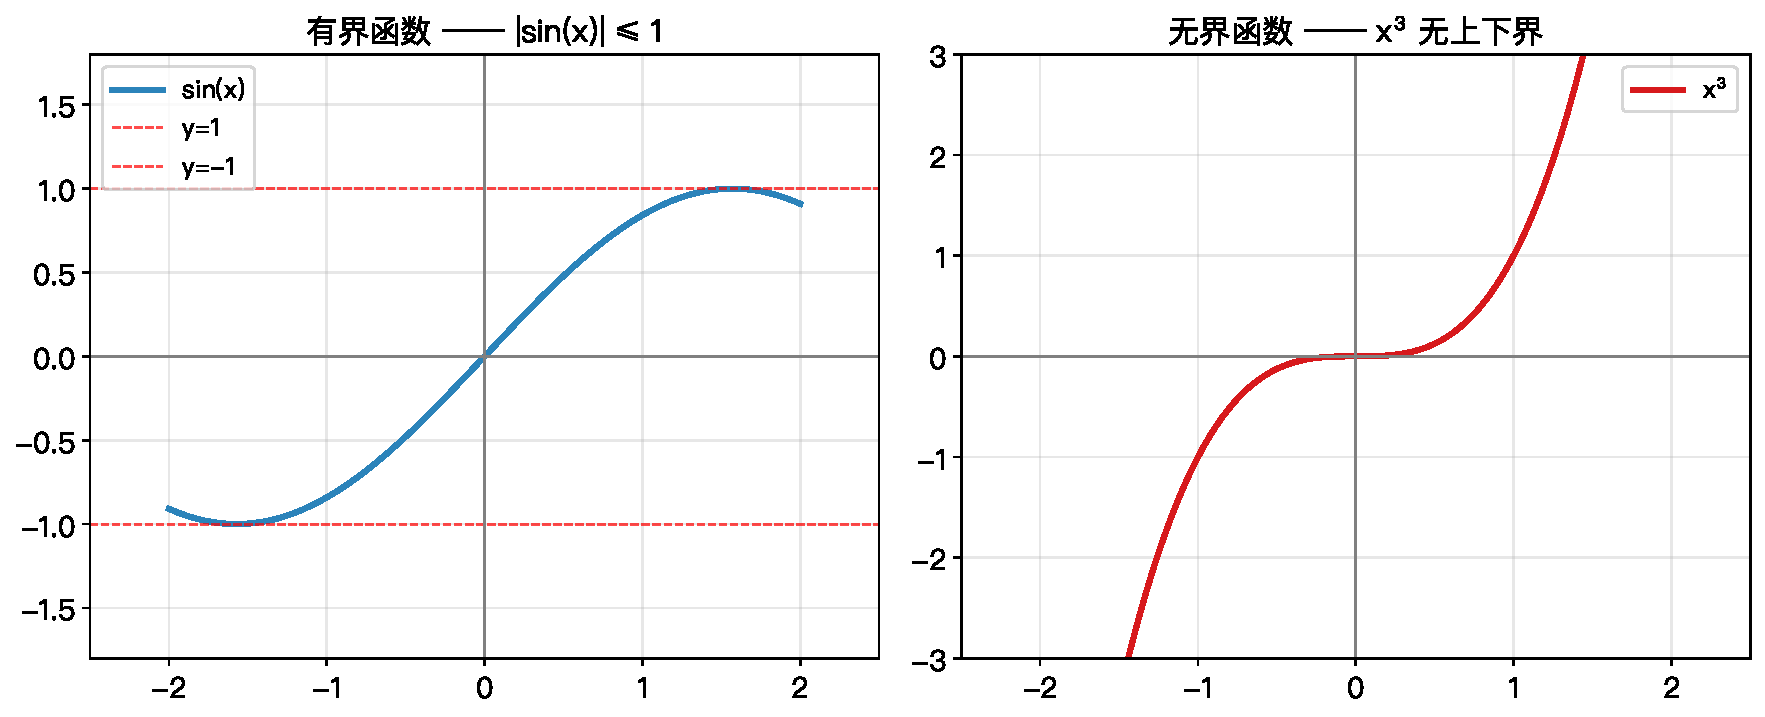
\includegraphics[width=0.85\textwidth]{figures/ch08_bounded.pdf}
\end{center}

\textbf{左图}（\(\sin x\)）：\(|\sin x| \le 1\)——有界函数，上下界为 \(\pm 1\)。\\
\textbf{右图}（\(x^3\)）：没有实数 \(M\) 能限制它——无界函数。

\textbf{常见有界函数：} \(\sin x\)、\(\cos x\)、\(\arctan x\)、常数函数

\textbf{常见无界函数：} \(x^n\)、\(a^x\)、\(\log_a x\)、\(\tan x\)
\end{examplebox}


% ============================================================
\section{复合函数——函数的函数}
% ============================================================

\begin{definitionbox}[复合函数]
如果 \(y = f(u)\)，且 \(u = g(x)\)，那么
\[
y = f(g(x))
\]
称为 \(f\) 和 \(g\) 的\textbf{复合函数}（读作 f of g of x）。

其中 \(g\) 是\textbf{内层函数}，\(f\) 是\textbf{外层函数}。
\end{definitionbox}

\begin{examplebox}[6——复合函数的例子]
\[
f(u) = \sqrt{u},\quad g(x) = 1 - x^2 \;\Longrightarrow\; f(g(x)) = \sqrt{1 - x^2}
\]

从外到内读：\(\sqrt{\;\cdot\;}\) 里面是 \(1 - x^2\)。

\textbf{复合函数的定义域：}
\begin{enumerate}
  \item 先找内层函数 \(g(x)\) 的定义域
  \item 再保证外层函数 \(f(u)\) 的定义域——即 \(g(x)\) 的值必须在 \(f\) 的定义域内
\end{enumerate}

\textbf{例：} \(f(x) = \sqrt{x}\)，\(g(x) = 2x - 1\)，则 \(f(g(x)) = \sqrt{2x - 1}\)。
定义域：\(2x - 1 \ge 0\)，即 \(x \ge 1/2\)。
\end{examplebox}


% ============================================================
\section{反函数——逆对应}
% ============================================================

\begin{definitionbox}[反函数]
如果函数 \(f: D \to R\) 是一一对应的（每个 \(y\) 唯一对应一个 \(x\)），
那么它的\textbf{反函数}（读作 fǎn hán shù）记作 \(f^{-1}\)：
\[
f^{-1}(y) = x \;\Longleftrightarrow\; f(x) = y
\]

\textbf{图像关系：} \(y = f(x)\) 和 \(y = f^{-1}(x)\) 关于直线 \(y = x\) 对称。
\end{definitionbox}

\begin{examplebox}[7——反函数的对称性]
\begin{center}
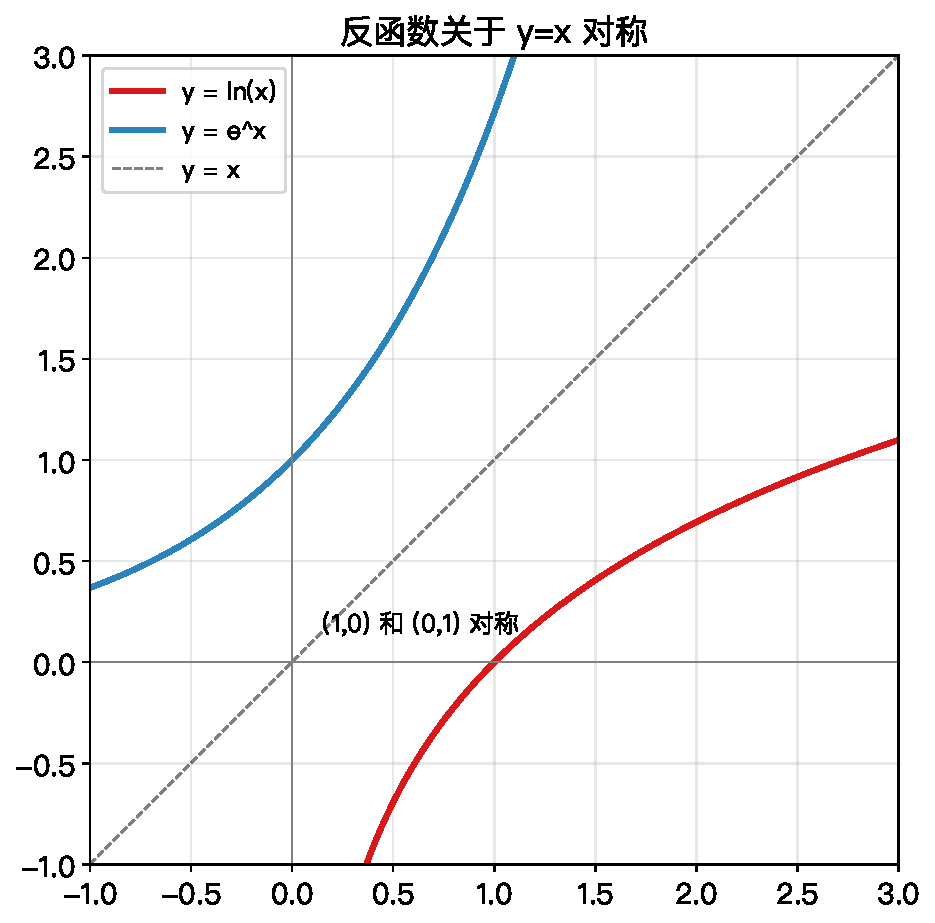
\includegraphics[width=0.5\textwidth]{figures/ch08_inverse_function.pdf}
\end{center}

\textbf{指数和对数是反函数：}
\[
y = e^x \;\Longleftrightarrow\; y = \ln x
\]
\((0,1)\) 在 \(e^x\) 上，\((1,0)\) 在 \(\ln x\) 上——关于 \(y = x\) 对称。

\textbf{另一对反函数：}
\[
y = x^2 \;(x \ge 0) \;\Longleftrightarrow\; y = \sqrt{x}
\]
\end{examplebox}

\begin{notebox}
\textbf{不是所有函数都有反函数！}
只有\textbf{一一对应}的函数才有反函数（即每个 \(y\) 值只对应一个 \(x\) 值）。

例如 \(y = x^2\)（定义域为 \(\mathbb{R}\)）没有反函数，因为 \(y=4\) 对应 \(x=2\) 和 \(x=-2\)。
但如果限制定义域为 \(x \ge 0\)，则有反函数 \(y = \sqrt{x}\)。
\end{notebox}


% ============================================================
\section{函数性质在 AI 中的应用}
% ============================================================

\begin{examplebox}[8——激活函数]
AI 中的激活函数需要特定的性质：

\begin{center}
\begin{tabular}{c|c|c}
\textbf{激活函数} & \textbf{数学形式} & \textbf{关键性质} \\
\hline
Sigmoid & \(\sigma(x) = \dfrac{1}{1 + e^{-x}}\) & 有界 \((0,1)\)，单调递增 \\
ReLU & \(\text{ReLU}(x) = \max(0, x)\) & 无上界，单调递增 \\
Tanh & \(\tanh x = \dfrac{e^x - e^{-x}}{e^x + e^{-x}}\) & 有界 \((-1,1)\)，奇函数 \\
\end{tabular}
\end{center}

\textbf{为什么需要这些性质？}
\begin{itemize}
  \item 有界性：把输出限制在特定范围（如概率在 0 到 1 之间）
  \item 单调性：保证梯度方向一致，训练更稳定
  \item 奇函数：某些情况下加速收敛（Tanh 比 Sigmoid 快）
\end{itemize}
\end{examplebox}


% ============================================================
\section{第0编总回顾——函数基础重建完成！}
% ============================================================

八章、从零开始，你走过了这样一条路：

\begin{center}
\fcolorbox{blue!40}{blue!5}{\parbox{0.9\textwidth}{
\textbf{\large 第0编 · 函数基础重建 · 路线图}

\[
\begin{array}{c}
\text{第1章 函数的概念（什么是函数？）} \\
\downarrow \\
\text{第2章 函数的图像（把函数画出来）} \\
\downarrow \\
\text{第3章 幂函数与多项式（幂的增长）} \\
\downarrow \\
\text{第4章 指数函数（指数增长）} \\
\downarrow \\
\text{第5章 对数函数（指数的逆）} \\
\downarrow \\
\text{第6-7章 三角函数（周期运动）} \\
\downarrow \\
\text{第8章 四大性质 + 复合与反函数（系统化总结）}
\end{array}
\]
}}
\end{center}

你不再是从零开始的初学者——你已经掌握了数学分析所需要的\textbf{全部预备知识}。


% ============================================================
\section{符号卡片}
% ============================================================

\begin{symbolcard}
单调递增 & —— & \(x_1 < x_2 \Rightarrow f(x_1) < f(x_2)\) \\
单调递减 & —— & \(x_1 < x_2 \Rightarrow f(x_1) > f(x_2)\) \\
奇函数 \(f(-x) = -f(x)\) & \verb|f(-x) = -f(x)| & 关于原点对称 \\
偶函数 \(f(-x) = f(x)\) & \verb|f(-x) = f(x)| & 关于 \(y\) 轴对称 \\
周期 \(T\) & —— & \(f(x + T) = f(x)\) \\
有界 \(|f(x)| \le M\) & —— & 存在常数 \(M\) 控制函数值 \\
\(f(g(x))\) & \verb|f(g(x))| & 复合函数，g 在内 f 在外 \\
\(f^{-1}(x)\) & \verb|f^{-1}(x)| & 反函数，与 \(f\) 关于 \(y=x\) 对称 \\
\end{symbolcard}


% ============================================================
\section{代码验证}
% ============================================================

\begin{lstlisting}[caption=函数性质的数值验证]
import numpy as np

# 1. 验证奇偶性
print("=== 奇偶性验证 ===")
def check_parity(f, name, xs):
    is_odd = all(abs(f(-x) + f(x)) < 1e-10 for x in xs)
    is_even = all(abs(f(-x) - f(x)) < 1e-10 for x in xs)
    if is_odd: print(f"  {name}: 奇函数")
    elif is_even: print(f"  {name}: 偶函数")
    else: print(f"  {name}: 非奇非偶")

xs = np.linspace(0.1, 5, 20)
check_parity(lambda x: x**3, "x^3", xs)
check_parity(lambda x: x**2, "x^2", xs)
check_parity(lambda x: np.sin(x), "sin(x)", xs)
check_parity(lambda x: np.cos(x), "cos(x)", xs)
check_parity(lambda x: 2**x, "2^x", xs)

print()

# 2. 验证周期性
print("=== 周期性验证 ===")
for T in [2*np.pi, np.pi]:
    x = 0.5
    print(f"  sin(x+{T:.2f}) = {np.sin(x+T):.4f}, sin(x) = {np.sin(x):.4f}")

print()

# 3. 验证有界性
print("=== 有界性验证 ===")
print(f"  sin(x) 的最大值: {np.max(np.sin(np.linspace(0, 100, 10000))):.4f}")
print(f"  sin(x) 的最小值: {np.min(np.sin(np.linspace(0, 100, 10000))):.4f}")
print(f"  arctan(x) 的最大值: {np.arctan(1e6):.4f}")
print(f"  arctan(x) 的最小值: {np.arctan(-1e6):.4f}")

print()

# 4. 验证反函数关系
print("=== 反函数验证 ===")
for x in [0.5, 1, 2, 3]:
    exp_val = np.exp(x)
    log_val = np.log(exp_val)
    print(f"  e^{x:.1f} = {exp_val:.4f}, ln(e^{x:.1f}) = {log_val:.4f}")
\end{lstlisting}

运行结果：
\begin{lstlisting}[frame=none,backgroundcolor={},numbers=none]
=== 奇偶性验证 ===
  x^3: 奇函数
  x^2: 偶函数
  sin(x): 奇函数
  cos(x): 偶函数
  2^x: 非奇非偶

=== 周期性验证 ===
  sin(x+6.28) = 0.4794, sin(x) = 0.4794
  sin(x+3.14) = -0.4794, sin(x) = 0.4794

=== 有界性验证 ===
  sin(x) 的最大值: 0.9999
  sin(x) 的最小值: -0.9999
  arctan(x) 的最大值: 1.5708
  arctan(x) 的最小值: -1.5708

=== 反函数验证 ===
  e^0.5 = 1.6487, ln(e^0.5) = 0.5000
  e^1.0 = 2.7183, ln(e^1.0) = 1.0000
  e^2.0 = 7.3891, ln(e^2.0) = 2.0000
  e^3.0 = 20.0855, ln(e^3.0) = 3.0000
\end{lstlisting}


% ============================================================
\section{本章小结}
% ============================================================

\begin{progressbox}
\textbf{四大性质：}
\begin{itemize}
  \item 单调性：递增 \((x_1 < x_2 \Rightarrow f(x_1) < f(x_2))\) 或递减
  \item 奇偶性：奇 \((f(-x) = -f(x))\)、偶 \((f(-x) = f(x))\)、或非奇非偶
  \item 周期性：\(f(x + T) = f(x)\)，常见周期 \(2\pi, \pi\)
  \item 有界性：存在 \(M\) 使 \(|f(x)| \le M\)
\end{itemize}

\textbf{复合函数：} \(f(g(x))\)——从内到外逐层计算

\textbf{反函数：} \(f^{-1}\)——关于 \(y = x\) 对称，只有一一对应才有反函数
\end{progressbox}

\subsection*{通往第一编——数列极限}

\textbf{第0编到此结束！} 你完成了函数基础重建的全部 8 章。

\textbf{第一编}我们将进入数学分析的核心——\textbf{数列极限}。
这是你第一次接触"无限"和"趋近"的严格数学语言。
准备好了吗？我们开始。


% ============================================================
% 习题
% ============================================================
\section{习题}

% ===== 送分 =====

\begin{exercise}[0]
判断 \(f(x) = x + 1\) 是单调递增还是递减？
\end{exercise}

\begin{exercise}[0]
判断 \(f(x) = 3\) 是奇函数、偶函数、还是非奇非偶？
\end{exercise}

\begin{exercise}[0]
\(\sin x\) 的周期是多少？\(\tan x\) 的周期是多少？
\end{exercise}

\begin{exercise}[0]
判断 \(f(x) = \arctan x\) 是有界函数还是无界函数？
\end{exercise}

% ===== 简单 =====

\begin{exercise}[1]
证明 \(f(x) = 3x - 2\) 是单调递增函数。
\end{exercise}

\begin{exercise}[1]
判断奇偶性：
\[
(1)\; f(x) = x^4 + 1 \qquad
(2)\; f(x) = x^3 + x \qquad
(3)\; f(x) = 2^x \qquad
(4)\; f(x) = |x|
\]
\end{exercise}

\begin{exercise}[1]
已知 \(f(x) = x^2\)，\(g(x) = 2x + 1\)，求 \(f(g(1))\) 和 \(g(f(1))\)。
\end{exercise}

\begin{exercise}[1]
\(y = \ln x\) 的反函数是什么？\(y = e^x\) 的反函数呢？
\end{exercise}

% ===== 基础 =====

\begin{exercise}[2]
求复合函数 \(f(g(x))\) 及其定义域：
\[
(1)\; f(x) = \sqrt{x},\; g(x) = x - 3 \qquad
(2)\; f(x) = \frac{1}{x},\; g(x) = x + 2
\]
\end{exercise}

\begin{exercise}[2]
证明 \(f(x) = x^2 + 1\) 在 \((-\infty, 0]\) 上单调递减，在 \([0, \infty)\) 上单调递增。
\end{exercise}

\begin{exercise}[2]
求下列函数的值域，并判断是否有界：
\[
(1)\; f(x) = \sin x - 1 \qquad (2)\; f(x) = e^{-x^2} \qquad (3)\; f(x) = \frac{1}{x}
\]
\end{exercise}

\begin{exercise}[2]
求函数 \(y = \sin(2x + \pi/3)\) 的周期、振幅、初相。
\end{exercise}

% ===== 普通 =====

\begin{exercise}[3]
已知 \(f(x) = 
\begin{cases}
x^2, & x \ge 0 \\
-x,  & x < 0
\end{cases}\)，判断 \(f(x)\) 的奇偶性。
\end{exercise}

\begin{exercise}[3]
已知 \(f(x) = \ln(x + \sqrt{1 + x^2})\)，证明 \(f(x)\) 是奇函数。
\end{exercise}

\begin{exercise}[3]
求下列函数的反函数：
\[
(1)\; f(x) = 3x + 2 \qquad (2)\; f(x) = \frac{x - 1}{x + 1} \;(x \neq -1)
\]
\end{exercise}

\begin{exercise}[3]
已知 \(f(x) = e^x\)，\(g(x) = \sin x\)，求 \(f(g(x))\) 和 \(g(f(x))\)，并说明它们分别是什么函数（幂/指/对/三角/复合）？
\end{exercise}

\begin{exercise}[3]
已知函数 \(f(x) = \log_2 (x^2 + 1)\)。
\begin{enumerate}
  \item[(1)] 求定义域
  \item[(2)] 判断奇偶性
  \item[(3)] 求值域（提示：\(x^2 + 1 \ge 1\)，所以 \(\log_2(x^2+1) \ge 0\)）
\end{enumerate}
\end{exercise}

% ===== 中等 =====

\begin{exercise}[4]
已知 \(f(x) = \dfrac{2^x - 2^{-x}}{2}\)（这其实是 \(\sinh x\)，双曲正弦）。
\begin{enumerate}
  \item[(1)] 判断奇偶性
  \item[(2)] 证明 \(f\) 是单调递增的
  \item[(3)] 求 \(f\) 的值域
\end{enumerate}
\end{exercise}

\begin{exercise}[4]
已知 \(f(x) = x^2 - 4x + 5\)。
\begin{enumerate}
  \item[(1)] 配方法写成 \(f(x) = (x - a)^2 + b\) 的形式
  \item[(2)] 判断单调区间（在哪个区间递增？哪个区间递减？）
  \item[(3)] 求最小值
\end{enumerate}
\end{exercise}

\begin{exercise}[4]
求函数 \(f(x) = \sqrt{1 - \sin^2 x}\) 的周期（提示：先化简）。
\end{exercise}

\begin{exercise}[4]
设 \(f(x) = \dfrac{1}{1 + e^{-x}}\)（Sigmoid 函数）。
\begin{enumerate}
  \item[(1)] 证明 \(f\) 是单调递增的
  \item[(2)] 证明 \(0 < f(x) < 1\)
  \item[(3)] 求 \(\lim_{x \to \infty} f(x)\) 和 \(\lim_{x \to -\infty} f(x)\)
\end{enumerate}
\end{exercise}

\begin{exercise}[4]
已知 \(f(x) = x^2 - 2x\)，\(g(x) = x + 1\)。
\begin{enumerate}
  \item[(1)] 求 \(f(g(x))\) 和 \(g(f(x))\)
  \item[(2)] 解方程 \(f(g(x)) = g(f(x))\)
\end{enumerate}
\end{exercise}

% ===== 进阶 =====

\begin{exercise}[5]
已知 \(f(x)\) 是奇函数，\(g(x)\) 是偶函数，且 \(f(x) + g(x) = e^x\)。
\begin{enumerate}
  \item[(1)] 用 \(x\) 替换为 \(-x\) 得到另一个方程
  \item[(2)] 联立解出 \(f(x)\) 和 \(g(x)\) 的表达式
\end{enumerate}
（提示：利用奇偶性：\(f(-x) = -f(x)\)，\(g(-x) = g(x)\)）
\end{exercise}

\begin{exercise}[5]
证明：若 \(f\) 和 \(g\) 都是单调递增函数，则 \(f(g(x))\) 也是单调递增函数。
\end{exercise}

\begin{exercise}[5]
求函数 \(y = \arctan \dfrac{1}{x}\)（\(x \neq 0\)）的值域。
\end{exercise}

\begin{exercise}[5]
已知 \(f(x) = \log_a (2 - ax)\)（\(a > 0, a \neq 1\)）在 \([0, 1]\) 上单调递减，求 \(a\) 的取值范围。
\end{exercise}

% ===== 拔高 =====

\begin{exercise}[6]
已知函数 \(f(x) = |x - 1| + 2|x - 2| + 3|x - 3|\)。
\begin{enumerate}
  \item[(1)] 去掉绝对值，写成分段函数
  \item[(2)] 求每个分段区间上的单调性
  \item[(3)] 求最小值
\end{enumerate}
\end{exercise}

\begin{exercise}[6]
求证：定义在 \(\mathbb{R}\) 上的任意函数 \(f(x)\) 都可以写成
一个奇函数和一个偶函数的和。
（提示：令 \(g(x) = \dfrac{f(x) + f(-x)}{2}\)，\(h(x) = \dfrac{f(x) - f(-x)}{2}\)）
\end{exercise}

\begin{exercise}[6]
已知函数 \(f(x)\) 满足 \(f(x + y) = f(x) + f(y)\) 对所有 \(x, y\) 成立。
\begin{enumerate}
  \item[(1)] 证明 \(f\) 是奇函数
  \item[(2)] 如果 \(f(1) = 2\)，求 \(f(5)\) 和 \(f(-3)\)
\end{enumerate}
\end{exercise}

% ===== 极难 =====

\begin{exercise}[7]
函数 \(f: \mathbb{R} \to \mathbb{R}\) 满足：
\[
f(x + y) + f(x - y) = 2f(x)\cos y \quad \text{对所有 } x, y \in \mathbb{R} \text{ 成立}
\]
\begin{enumerate}
  \item[(1)] 令 \(y = 0\)，求 \(f(0)\)
  \item[(2)] 令 \(x = 0\)，证明 \(f\) 是偶函数
  \item[(3)] 令 \(x = \pi/2\)，证明 \(f\) 是周期函数
  \item[(4)] 结合 \(f(\pi/2) = 1\)，求 \(f(0)\)、\(f(\pi)\)、\(f(2\pi)\)
\end{enumerate}

\textbf{说明：} 这道题是函数方程与函数性质的综合——从给定的方程中，
一步步推导出函数的奇偶性、周期性、特殊值。
这是数学分析中"由性质确定函数"的一个经典范例。
\end{exercise}
